\section{非自治系统稳定性的概念}\label{3Bref}
考虑非自治系统的自由运动
\begin{equation}\label{freeofnonauto}
  \dot{x}=f(t,x)
\end{equation}
其中$f : [0, \infty) \times D \rightarrow \R{}^n$是从$[0, \infty) \times D$至$\R{}^n$的映射,它对$t$分段连续,对$x$局部Lipschitz。$D\subset\R{}^n$为包含$x=0$的域。若$f(t,0)\equiv0,\forall t\ge t_0$,则$x=0$为$t=t_0$时刻的平衡点。
\begin{definition}[非自治系统的稳定性]
 系统 \eqref{freeofnonauto} 的平衡点 $x = 0$是
  \begin{itemize}[leftmargin=1em]
    \item {\bf 稳定的(stable)}\index{稳定的(stable)},若对每个$\varepsilon > 0$,都存在 $\delta =    \delta (\varepsilon, t_0)>0$使得
    \begin{equation}
      \| x (t_0) \| < \delta \quad \Rightarrow \quad \| x (t) \| <
      \varepsilon, \forall t \geq t_0 \geq 0 \label{Nonauto:stable:def} .
    \end{equation}
    \item {\bf 不稳定的(unstable)}\index{不稳定的(unstable)},若其不是稳定的。
    
    \item {\bf 一致稳定的(uniformly stable,US)}\index{稳定的(stable)!一致$\sim$(uniformly)},若对每个$\varepsilon > 0$,都存在
    $\delta = \delta (\varepsilon) > 0$(与$t_0$无关),使得 \eqref{Nonauto:stable:def} 成立。
    
    \item {\bf 渐近稳定的(asymptotically stable,AS)}\index{稳定的(stable)!渐近$\sim$(asymptotically)},若其是稳定的,且存在一正数
     $c = c (t_0)$ 使得
    \begin{equation}
      \forall \| x (t_0) \| < c, \lim_{t \rightarrow \infty} x (t) = 0 \label{Nonauto:astable:def} .
    \end{equation}
    \item {\bf 一致渐近稳定的(uniformly asymptotically stable)},\index{稳定的(stable)!一致渐近$\sim$(uniformly asymptotically,UAS)}若其为一致稳定的,且存在一正常数 $c$(与$t_0$无关)使得 \eqref{Nonauto:astable:def} 成立;换言之,对任意$\eta>0$,都存在$T=T(\eta)>0$使
    \[\|x(t)\|<\eta,\forall t\ge t_0+T(\eta),\forall\|x(t_0)\|<c\]
    
    \item {\bf 全局一致渐近稳定的(globally uniformly asymptotically stable,GUAS)}\index{稳定的(stable)!全局一致渐近$\sim$(globally uniformly asymptotically)},若其是一致稳定的,\eqref{Nonauto:stable:def} 中的$\delta(\varepsilon)$满足$\lim\limits_{\varepsilon\to\infty}\delta(\varepsilon)=\infty$,且对于任意正数$\eta$和$c$,都存在$T=T(\eta,c)>0$使得
    \[\|x(t)\|<\eta,\forall t\ge t_0+T(\eta,c),\forall\|x(t_0)\|<c\]
  \end{itemize}
\end{definition}
\begin{note}
  “一致”是说初始时刻任意性,“全局”则是说初始状态任意性。一致渐近稳定,通俗地说,就是只要时间足够长,状态总能进入给定的离原点足够近的范围(渐近),
  并且经过的时间$T$仅与所要求的状态与原点的距离有关($T(\eta)$),而与初始时刻无关(一致);全局一致渐近稳定,则是在此基础上加入了“全局”的要求,也即初始状态任意($c$能取遍所有的正数)。达到与原点给定距离之内的用时$T$,仍然与初始时刻无关,
  不过增加了对初始状态的相关性($T(\eta,c)$)——很容易理解:不能要求“很远”的初始状态与“很近”的初始状态有相同的过渡时间。%真的假的?来点最速降线(
\end{note}
\begin{example}[稳定但不一致稳定]
  考虑如下非线性系统
  \[ \dot{x} = (6 t  \sin  t - 2 t) x \]
  其解为
  \begin{align*}
    x (t) & =  x (t_0) \exp \left\{ \int^t_{t_0} (6 \tau \sin \tau - 2 \tau)
    \diff \tau \right\}\\
    & =  x (t_0) \exp \{ 6 \sin  t - 6 t  \cos  t - t^2 - 6 \sin  t_0 + 6
    t_0 \cos  t_0 + t^2_0 \}
  \end{align*}
  注意到 $6 \sin  t - 6 t  \cos  t - t^2 \leq 6 + 6 t - t^2 = - (t - 3)^2 + 15
  \leq 15$.
  
  选 $c (t_0) = \exp (15 - 6 \sin  t_0 + 6 t_0 \cos  t_0 + t^2_0)$,则有 $\| x (t) \| \leq \| x (t_0) \| \cdot c (t_0), \forall t
  \geq t_0 \geq 0$.
  
  对于任意 $\varepsilon > 0$,选取 $\delta = \frac{\varepsilon}{c (t_0)}$,即得
  \[ \| x (t_0) \| < \delta = \frac{\varepsilon}{c (t_0)} \quad \Rightarrow
     \quad \| x (t) \| \leq \| x (t_0) \| \cdot c (t_0) < \frac{\varepsilon}{c
     (t_0)} \cdot c (t_0) = \varepsilon \]
  这也就表明了原点是稳定的。
  
  下面看看当$t_0$变化时,方程的解对其是否敏感。

  令 $t_0 = 2 k \pi$。考察$x (t)$在$t = t_0 + \pi = (2 k + 1)\pi$时刻的取值:
  \begin{align*}
    x (t_0 + \pi) & =  x (t_0) \exp \{ 6 \sin [(2 k + 1) \pi] - 6 (2 k + 1)
    \pi \cos [(2 k + 1) \pi] - [(2 k + 1) \pi]^2 \\
    &  \quad - 6 \sin (2 k \pi) + 6 (2 k \pi) \cos (2 k \pi) - (2 k \pi)^2 \} \\
    & =  x (t_0) \exp \{ 6 (2 k + 1) \pi - [(2 k + 1) \pi]^2  + 12 k \pi -
    (2 k \pi)^2 \} \\
    & =  x (t_0) \mathrm{e}^{\left( \text{} 4 k + 1 \right) (6 - \pi) \pi}
  \end{align*}
  则$k \rightarrow\infty$时
  \[ \frac{x (t_0 + \pi)}{x (t_0)} = \mathrm{e}^{\left( \text{} 4 k + 1 \right) (6 -
     \pi) \pi} \rightarrow \infty,  \]
  因此,$t_0$离$0$越远,其解的变化就越剧烈,
  则对于任意 $\varepsilon > 0$,不存在与$t_0$ 无关的$\delta (\varepsilon)$,也就不满足一致稳定的定义。
\end{example}
\newpage
下面的引理利用比较函数,给出了一致稳定和一致渐近稳定的更为简洁明了的定义。
\begin{lemma}\label{comp_uniform}
  系统 \eqref{freeofnonauto} 的平衡点 $x = 0$是
  \begin{itemize}[leftmargin=1em]
  \item 一致稳定的\index{稳定的(stable)!一致$\sim$(uniformly)},若存在一$\mathcal{K}$类函数 $\alpha$和正常数$c$(与$t_0$无关)\index{K@$\mathcal{K}$ 类函数}使得
   \[ \| x (t) \| \leq \alpha (\| x (t_0) \|), \forall t \geq t_0 \geq 0,
       \forall \| x (t_0) \| \le c. \]
  \item 一致渐近稳定的\index{稳定的(stable)!一致渐近$\sim$(uniformly asymptotically)},若存在一$\mathcal{K}\mathcal{L}$ 类函数 $\beta$ 和正常数$c$(与$t_0$无关),\index{Kl@$\mathcal{K}\mathcal{L}$ 类函数}使得
  \begin{equation}
    \| x (t) \| \leq \beta (\| x (t_0) \|, t - t_0), \forall t \geq t_0 \geq
    0, \forall \| x (t_0) \| \le  c \label{uas:iff:kl} .
  \end{equation}
  \item 全局一致渐近稳定的\index{稳定的(stable)!全局一致渐近$\sim$(globally uniformly asymptotically)},若不等式 \eqref{uas:iff:kl} 对所有初始状态$x (t_0)$都成立,即$c$可取至$\infty$。
  \item 一致指数稳定的,若上述$\beta$具有$\beta(r,t)=kr\mathrm{e}^{-\lambda t}$($k>0,\lambda>0$)的形式:
  \[\|x(t)\|\le k\|x(t_0)\|\mathrm{e}^{-\lambda(t-t_0)}, \forall t \geq t_0,\forall \| x (t_0) \| \le  c \]
  \end{itemize}
\end{lemma}
\begin{example}[一致稳定且渐近稳定,但非一致渐近稳定]
  考虑下面系统
  \[\dot{x}=\frac{-x}{1+t},t>-1\]
  可求得其解为
  \begin{align*}
    x(t)=x(t_0)\mathrm{e}^{\int_{t_0}^t\frac{-1}{1+s}\diff s}=x(t_0)\mathrm{e}^{\ln(1+s)|_t^{t_0}}
    =x(t_0)\mathrm{e}^{\ln\frac{1+t_0}{1+t}}=x(t_0)\frac{1+t_0}{1+t}
  \end{align*}
  可见,$\|x(t)\|\le\|x(t_0)\|$,在 \ref{comp_uniform} 第一条中取$\alpha(r)=r$,即可说明原点是一致稳定的。

  \begin{wrapfigure}{R}{0.36\textwidth}
    \vspace{-1em}
  	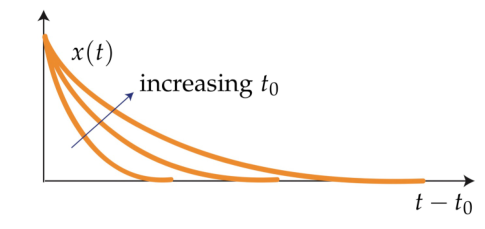
\includegraphics[width=0.95\linewidth]{./figure/nonlinear/not_uniform.png}
    \captionof{figure}{随$t_0$增长,收敛越来越慢}
  \end{wrapfigure}

  \vspace{1em}
  原点也是渐近稳定的(随时间增长$x(t)\to0$),但并非一致渐近稳定,因为考虑下式(绘出示意图如右)
  \[x(t)=x(t_0)\frac{1+t_0}{1+t_0+(t-t_0)}=\frac{x(t_0)}{1+\frac{t-t_0}{1+t_0}}\]
  即可发现收敛的速率与$t_0$有关。
  % \begin{center}
  %   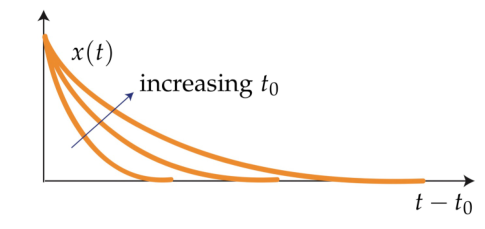
\includegraphics[scale=0.3]{figure/nonlinear/not_uniform.png}
  %   \captionof{figure}{随$t_0$增长,收敛越来越慢}
  % \end{center}
\end{example}


